
%opening
\title{Konstruktion Ranking}
\author{Lothar Mödl}

\section{Ranking Sequenzdiagramm}

\begin{figure}
	\centering
	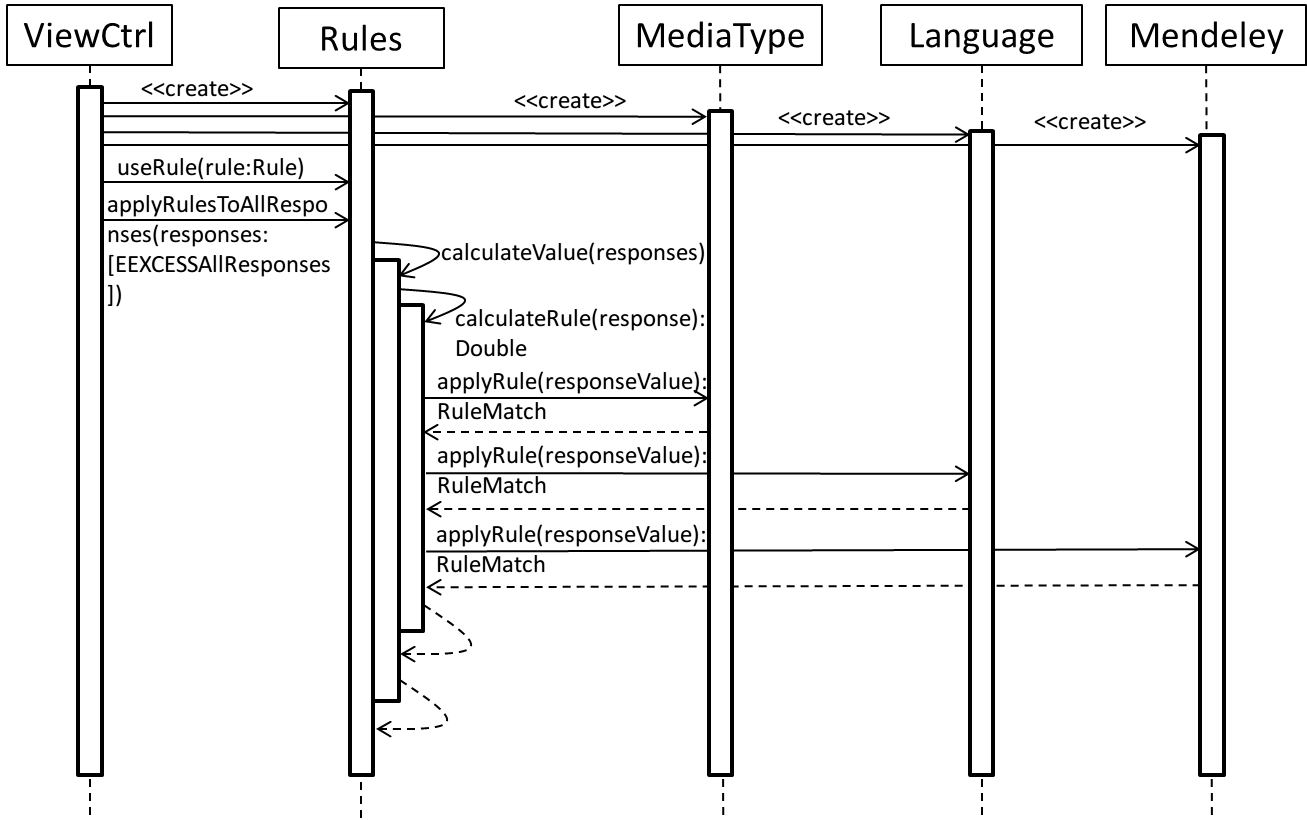
\includegraphics[width=12cm]{Sequenzdiagramm_Ranking}
	\caption{Sequenzdiagramm des Rankings}
	\label{fig:Ranking Sequenzdiagramm}
\end{figure}

Dieses Sequenzdiagramm zeigt einen exemplarischen Durchlauf des Rankings der Vorschläge für den Benutzer. Nachdem die Daten aus dem Internet abgerufen wurden und an den ViewController (Team UI) übergeben wurden folgt die Sortierung der Ergebnisse nach den Interessen des Nutzers. Es existieren eine Reihe an verschiedenen Regeln, die angewendet werden können. Die Anzahl an Regeln kann variieren. Welche Regeln angewendet werden, wird vom ViewController festgelegt mit Hilfe der Methode „useRule(rule:Rule)“. Nachdem die Regeln, die angewendet werden sollen, festgelegt wurden, müssen diese angewendet werden. Dies geschieht mit der Methode „applyRulesToAllResponses(responses:[EEXCESSAlllResponses])“. Als Argument müssen alle zuvor erhaltenen Ergebnisse mit übergeben werden. Die Klasse Rules übernimmt im Anschluss die Berechnungen, die für das Ranking der Ergebnisse notwendig sind. Die Methode „calculateValue(responses)“ berechnet in Verbindung mit der Methode „calculateRule(response): Double“ einen Durchschnittswert für jede einzelne Antwort für jeden einzelnen \SEARCH-Tag, nachdem jede Regel angewendet wurde. Eine Regeln wird durch den Aufruf der Methode „applyRule(responseValue): RuleMatch“ angewandt, welche jede Regel besitzt und liefert den Wert 0 oder 1 zurück. Dieser bedeutet, ob die Regel auf die Interessen des Nutzers zutrifft oder nicht. Zum Abschluss des Rankings werden die einzelnen Ergebnisse entsprechend nach dem zuvor errechneten Durchschnittswert sortiert. Im Anschluss erhält das Team UI die sortierten Werte zurück und kann sie dem Nutzer darstellen. 

\pagebreak

\section{Ranking Klassendiagramm}

\begin{figure}
	\centering
	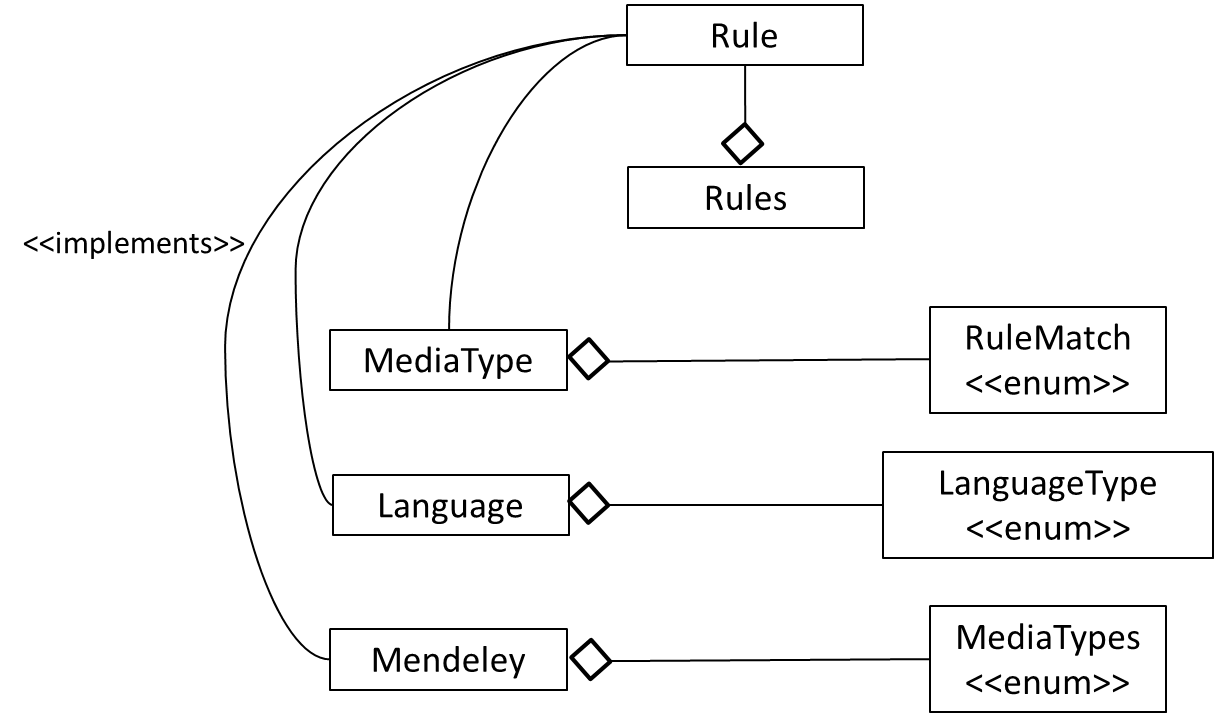
\includegraphics[width=12cm]{Klassendiagramm_Ranking}
	\caption{Klassendiagramm des Rankings}
	\label{fig:Ranking Klassendiagramm}
\end{figure}

\pagebreak

\section{Abruf der Daten vom Server Sequenzdiagramm}

Dieses Sequenzdiagramm zeigt einen exemplarischen Ablauf zum Abrufen der Daten vom Server. Zuerst wird eine Instanz des TaskControllers erzeugt. Dieser stellt die Schnittstelle zum View zur Verfügung. Er empfängt und sendet Daten von bzw. an den View. Die Methode „getRecommendations([SEARCHModel], setRecommendations:(String, [Response]))“ bildet die Schnittstelle, bei der die einzelnen, aus der HTML Seite ausgelesenen, SEARCH-Tags in Form von SEARCHModels übergeben werden, sowie die Methode „setRecommendations(String, [Responses])“, die für die Rückgabe der heruntergeladen Ergebnisse zuständig ist. Im Anschluss wird eine Instanz des JSONConnectionControllers sowie des EEXCESSRecommendationJSONControllers erzeugt. Der JSONConnectionCtrl ist für den Aufbau der Verbindung zum Server zuständig. Beim Erzeugen es EEXCESSRecommendationJSONControllers werden die SEARCHModels in einen JSON String konvertiert. Mit Hilfe der Methode „post(AnyObject, String, postCompleted(Bool, NSData))“ wird zuvor erzeugte JSON String an den Server gesendet. Nach Erhalt der Daten wird die Methode postCompleted(Bool, NSData) mit diesen heruntergeladenen Daten aufgerufen. Innerhalb von 
postCompleted(...) wird wiederum eine Instanz des EEXCESSRecommendationControllers erzeugt, welcher die JSON Daten parst und in die interne Struktur der App überführt. Hierfür wird für jede einzelne Antwort eines \SEARCH-Tags eine Instanz von EEXCESSSingleResponse erzeugt. Alle Antworten, die zu einem \SEARCH-Tag gehören, werden in einer neuen Instanz von EEXCESSAllResponses gespeichert.  Das komplette Array von allen EEXCESSAllResponses wird an den TaskCtrl zurückgegeben. Dieses Array wird mit der zu Beginn erhaltenen Methode „setRecommendations(String, [EEXCESSAllResponses])“ an den View zurückgegeben, welcher die Ergebnisse dann darstellt. 

\begin{figure}
	\centering
	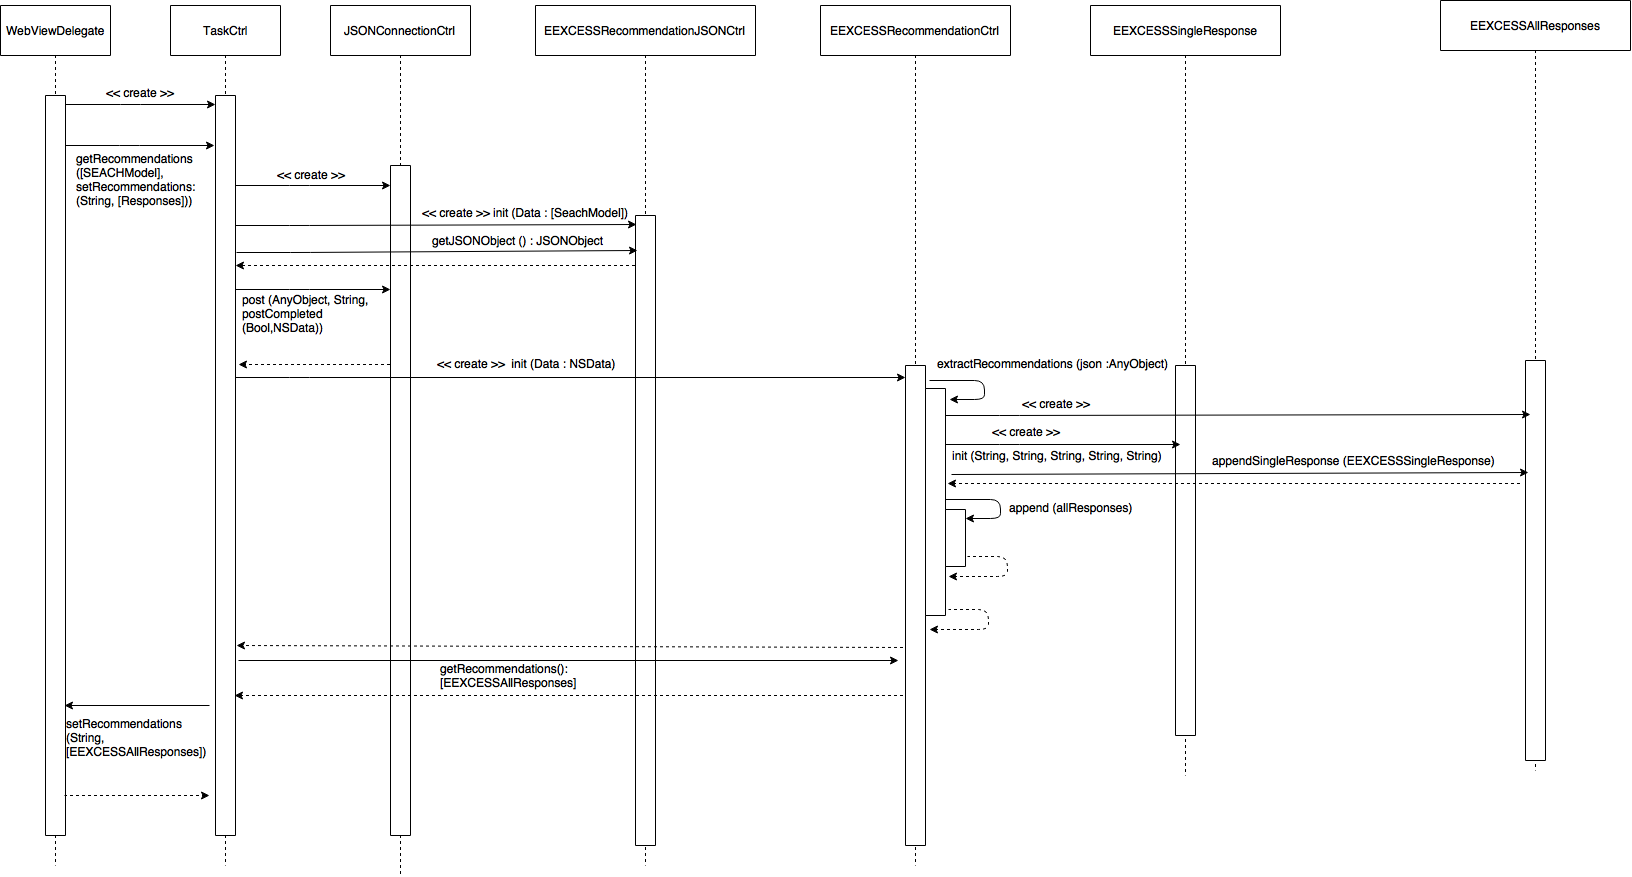
\includegraphics[width=12cm]{Sequenzdiagramm_Anfragen}
	\caption{Sequenzdiagramm einer Serveranfrage}
	\label{fig:Anfrage Sequenzdiagramm}
\end{figure}

\pagebreak

\section{Abruf der Daten vom Server Klassendiagramm}

\begin{figure}
	\centering
	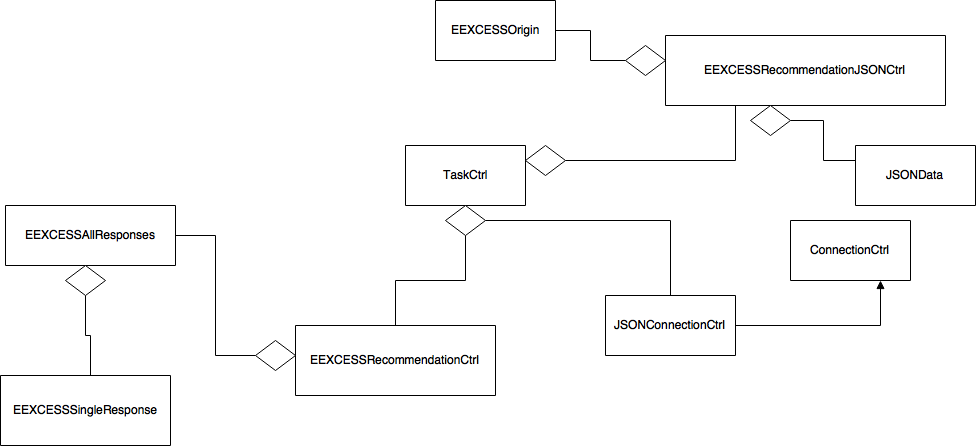
\includegraphics[width=12cm]{Klassendiagramm_Anfrage}
	\caption{Klassendiagramm einer Serveranfrage}
	\label{fig:Anfrage Klassendiagramm}
\end{figure}

\pagebreak
